%%%%%%%%%%%%%%%%%%%%%%%%%%%%%%%%%%%%%%%%%
% Short Sectioned Assignment
% LaTeX Template
% Version 1.0 (5/5/12)
%
% This template has been downloaded from:
% http://www.LaTeXTemplates.com
%
% Original author:
% Frits Wenneker (http://www.howtotex.com)
%
% License:
% CC BY-NC-SA 3.0 (http://creativecommons.org/licenses/by-nc-sa/3.0/)
%
%%%%%%%%%%%%%%%%%%%%%%%%%%%%%%%%%%%%%%%%%

%----------------------------------------------------------------------------------------
%	PACKAGES AND OTHER DOCUMENT CONFIGURATIONS
%----------------------------------------------------------------------------------------

\documentclass[paper=a4, fontsize=11pt]{scrartcl} % A4 paper and 11pt font size
\usepackage[brazilian]{babel}
\usepackage[utf8]{inputenc}
\usepackage[T1]{fontenc}
\usepackage{amsmath,amsfonts,amsthm,mathtools} % Math packages
\usepackage{xspace}
\usepackage{indentfirst}
\usepackage{placeins}


\usepackage{tikz}
\usetikzlibrary{arrows}
\usetikzlibrary{positioning}
\usetikzlibrary{calc}

%\usepackage{sectsty} % Allows customizing section commands
%\allsectionsfont{\centering \normalfont\scshape} % Make all sections centered, the default font and small caps

\usepackage{fancyhdr}
\pagestyle{fancyplain}
%\fancyhead{}
\fancyfoot[L]{} % Empty left footer
\fancyfoot[C]{} % Empty center footer
\fancyfoot[R]{\thepage} % Page numbering for right footer
\renewcommand{\headrulewidth}{0pt} % Remove header underlines
\renewcommand{\footrulewidth}{0pt} % Remove footer underlines
\setlength{\headheight}{13.6pt} % Customize the height of the header

\bibliographystyle{apalike}

%\sectionfont{\bfseries\Large\raggedright}
%\subsectionfont{\bfseries\Large\raggedright}

\newtheorem{theorem}{Teorema}
\newtheorem{definition}{Definição}
\newtheorem{property}{Propriedade}
\newtheorem{proposition}{Proposição}

\newenvironment{example}[1][Exemplo]{\begin{trivlist}
\item[\hskip \labelsep {\bfseries #1}]}{\end{trivlist}}
\newenvironment{exerc}[1][Exercício]{\begin{trivlist}
\item[\hskip \labelsep {\bfseries #1}]}{\end{trivlist}}


\numberwithin{equation}{subsection}
\numberwithin{figure}{subsection}
\numberwithin{table}{subsection}
\numberwithin{definition}{subsection}
\numberwithin{theorem}{subsection}
\numberwithin{property}{subsection}
\numberwithin{proposition}{subsection}
%\numberwithin{example}{subsection}

\numberwithin{equation}{section}
\numberwithin{figure}{section}
\numberwithin{table}{section}
\numberwithin{definition}{section}
\numberwithin{theorem}{section}
\numberwithin{property}{section}
\numberwithin{proposition}{section}
%\numberwithin{example}{section}

\def\ind{\perp\!\!\!\perp}
\def\nind{\not\!\perp\!\!\!\perp}

% Default fixed font does not support bold face
\DeclareFixedFont{\ttb}{T1}{txtt}{bx}{n}{12} % for bold
\DeclareFixedFont{\ttm}{T1}{txtt}{m}{n}{12}  % for normal

% Custom colors
\usepackage{color}
\definecolor{deepblue}{rgb}{0,0,0.5}
\definecolor{deepred}{rgb}{0.6,0,0}
\definecolor{deepgreen}{rgb}{0,0.5,0}

\usepackage{listings}

% Python style for highlighting
\newcommand\pythonstyle{\lstset{
language=Python,
basicstyle=\ttm,
otherkeywords={self},             % Add keywords here
keywordstyle=\ttb\color{deepblue},
emph={MyClass,__init__},          % Custom highlighting
emphstyle=\ttb\color{deepred},    % Custom highlighting style
stringstyle=\color{deepgreen},
frame=tb,                         % Any extra options here
showstringspaces=false            % 
}}

% Python environment
\lstnewenvironment{python}[1][]
{
\pythonstyle
\lstset{#1}
}
{}


%\setlength{•}{•}\parindent{0pt} % Removes all indentation from paragraphs - comment this line for an assignment with lots of text

%----------------------------------------------------------------------------------------
%	TITLE SECTION
%----------------------------------------------------------------------------------------

\newcommand{\horrule}[1]{\rule{\linewidth}{#1}} % Create horizontal rule command with 1 argument of height

\title{	
\normalfont \normalsize 
\textsc{Modelos Probabilísticos Baseados em Grafos} \\ 
\textsc{Prof. Denis Mauá} \\ [25pt]
%\horrule{0.5pt} \\[0.4cm] % Thin top horizontal rule
\huge Redes de Markov\\ [25pt]
%\horrule{1pt} \\[0.5cm] % Thick bottom horizontal rule
}
\author{Thales A. B. Paiva \\ thalespaiva@gmail.com} % Your name
\date{\today} % Today's date or a custom date

\renewcommand{\P}{\mathbb{P}}
\renewcommand{\bar}[1]{\overline{#1}}
\newcommand{\set}[1]{\mathcal{#1}}

\begin{document}


\maketitle % Print the title
\horrule{1pt} \\[0.5cm] % Thick bottom horizontal rule

\tableofcontents

\pagebreak
\section{Exercícios Teóricos}

\begin{exerc}
Prove que as seguintes afirmações são equivalentes para dois nós $X$ e $Y$ num DAG $\set{G}$:
\begin{enumerate}
  \item $X$ e $Y$ são adjacentes.
  \item Não há conjunto $\set{Z}$, com $X, Y \notin \set{Z}$, que d-separa $X$ e $Y$.
  \item $X$ e $Y$ não são d-separados por nenhum $(\text{an}(X) \cup \text{an}(Y))\setminus \{X, Y\}$.
  \item $X$ e $Y$ não são d-separados por $(\text{pa}(X) \cup \text{pa}(Y))\setminus \{X, Y\}$.
\end{enumerate}
\end{exerc}
\emph{Note que mudei um pouco as afirmações para $\set{Z}$ não conter $\{X, Y\}$. Isso pois a definição de d-separação considera que se $X \in \set{Z}$, então $\set{Z}$ d-separa $X$ e $Y$.}

\emph{Demonstração.}

\par{$1 \Rightarrow 2$}. 
Suponha que $X$ e $Y$ são nós adjacentes num DAG que são bloqueados por um conjunto $Z$ de vértices, a que nem $X$ nem $Y$ pertencem. Pela definição de bloqueio, a trilha $X \rightleftharpoons Y$ só pode ser bloqueada se $X \in \set{Z}$ ou se $Y \in \set{Z}$. Porém ambas contradizem nossas hipóteses, então não há conjunto que bloqueia a trilha $X \rightleftharpoons Y$. Portanto $X$ e $Y$ não podem ser d-separados, a menos que $X$ ou $Y$ faça parte do conjunto separador.

\par{$2 \Rightarrow 3$}.
Se não há conjunto que não contém $\{X, Y\}$ que d-separa $X$ e $Y$, então estes nós não podem ser d-separados por $(\text{an}(X) \cup \text{an}(Y))\setminus \{X, Y\}$.

\par{$3 \Rightarrow 4$}.
Suponha que $X$ e $Y$ não são d-separados por $(\text{an}(X) \cup \text{an}(Y))\setminus \{X, Y\}$. Então, como $(\text{pa}(X) \cup \text{pa}(Y))\setminus \{X, Y\} \subseteq (\text{an}(X) \cup \text{an}(Y))\setminus \{X, Y\}$, claro que $X$ e $Y$ não são d-separados por $(\text{pa}(X) \cup \text{pa}(Y))\setminus \{X, Y\}$.

\par{$4 \Rightarrow 1$}.
Suponha que $X$ e $Y$ não são d-separados por $P := (\text{pa}(X) \cup \text{pa}(Y))\setminus \{X, Y\}$. Então, ou $X$ e $Y$ são adjacentes, ou existe um descendente de $X$ e de $Y$ que está em $P$, para permitir que haja troca de informação entre $X$ e $Y$ através de uma estrutura em v. Mas, se existir um descendente de $X$ e de $Y$ que também é pai de $X$ ou de $Y$, então há um ciclo no DAG, o que é proibido. Logo, $X$ e $Y$ são adjacentes. 


\begin{exerc}
Suponha que seja dado um oráculo que responde a perguntas do tipo: 
$$
X \ind Y | Z?. 
$$
Descreva um algoritmo para decidir qual dos grafos da Figura~\ref{fig:grafos_ex2} representa as relações de independência induzida pelo oráculo, denotado por $I$.

\end{exerc}
\begin{figure}[hbtp]
\centering
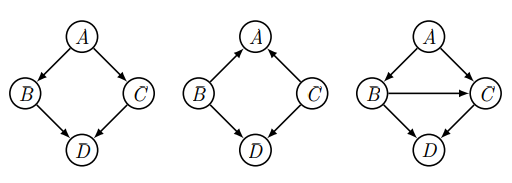
\includegraphics[scale=0.7]{images/exerc2_graphs.png}
\caption{Grafos para o exercício 2}
\label{fig:grafos_ex2}
\end{figure}

\emph{Considerei que certamente um dos grafos representa $I$.}

\emph{Resposta.} Primeiro pergunte ao oráculo se $B \ind C | \emptyset $. Se sim, então o segundo grafo representa $I$. Se não, então pergunte se $B \ind C | A$. Se sim, então o primeiro representa $I$. Se não, então $I$ é representado pelo terceiro grafo.

\end{document}